%============================ MAIN DOCUMENT ================================
% define document class
\PassOptionsToPackage{table}{xcolor}
\documentclass[
  a4paper,
  BCOR=15mm,            % Binding correction
  twoside,
  bibliography=totoc,   % If enabled add bibliography to TOC
  listof=totoc,         % If enabled add lists to TOC
  monolingual,
  invert-title,
]{bfhpub}

\LoadBFHModule{listings,terminal,boxes}


%---------------------------------------------------------------------------
% Documents paths
%---------------------------------------------------------------------------
\makeatletter
\def\input@path{{content/}}
%or: \def\input@path{{/path/to/folder/}{/path/to/other/folder/}}
\makeatother

%-----------------  Base packages     --------------------------------------
% Include Packages
\usepackage[main=english]{babel}  % https://www.namsu.de/Extra/pakete/Babel.html
%% To disable the french list setting you can add -- see https://gitlab.ti.bfh.ch/bfh-latex/bfh-ci/-/issues/166
%\frenchsetup{StandardLists=true}

\usepackage{amsmath}          % various features to facilitate writing math formulas
\usepackage{amsthm}           % enhanced version of latex's newtheorem
\usepackage{amsfonts}         % set of miscellaneous TeX fonts that augment the standard CM
\usepackage{amssymb}          % mathematical special characters

\usepackage{siunitx}

\usepackage{graphicx}         % integration of images
\usepackage{float}            % floating objects

\usepackage{caption}          % for captions of figures and tables
\usepackage{subcaption}       % for subcaptions in subfigures
\usepackage{cite}             % use bibtex
\usepackage{wrapfig}

\usepackage{exscale}          % mathematical size corresponds to textsize
\usepackage{multirow}         % multirow emables combining rows in tables
\usepackage{multicol}

\usepackage{longtable}

\usepackage{parskip}

% Setting Better font
\usepackage{lmodern}
\setmainfont{Latin Modern Sans}


%---------------------------------------------------------------------------
% Graphics paths
%---------------------------------------------------------------------------
\graphicspath{{pictures/}{figures/}}


%---------------------------------------------------------------------------
% Blind text -> for dummy text
%---------------------------------------------------------------------------
\usepackage{blindtext}
\usepackage{letltxmacro}
\LetLtxMacro{\blindtextblindtext}{\blindtext}

\RenewDocumentCommand{\blindtext}{O{\value{blindtext}}}{
	\begingroup\color{BFH-Gray}\blindtextblindtext[#1]\endgroup
}


%---------------------------------------------------------------------------
% Makeindex Package
%---------------------------------------------------------------------------
\usepackage{makeidx}
\makeindex
%\usepackage{imakeidx}          % To produce index
%\makeindex[columns=2,intoc]    % Index-Initialisation
%\makeindex[columns=3,columnseprule,columnsep,intoc]


%---------------------------------------------------------------------------
% Hyperref Package (Create links in a pdf)
%---------------------------------------------------------------------------
\usepackage[
	,bookmarks
	,plainpages=false
	,pdfpagelabels
        ,pdfusetitle
	,backref = {false}          % No index backreference
	,colorlinks = {true}        % Color links in a PDF
	,hypertexnames = {true}     % no failures "same page(i)"
	,bookmarksopen = {true}     % opens the bar on the left side
	,bookmarksopenlevel = {0}   % depth of opened bookmarks
	,linkcolor=.
	,filecolor=.
	,urlcolor=.
	,citecolor=.
]{hyperref}


%---------------------------------------------------------------------------
% Setup equation sets
%---------------------------------------------------------------------------
\newcounter{equationset}
\newcommand{\equationset}[1]{						% \equationset{<caption>}
	\refstepcounter{equationset}					% Step counter
	\begin{tabularx}{\textwidth}{l X}
	\footnotesize\color{BFH-Gray} \textbf{Equation set~\theequationset:} & \footnotesize\color{BFH-Gray} #1 % Print caption
	\end{tabularx}
}


%---------------------------------------------------------------------------
% Setup definitions
%---------------------------------------------------------------------------
\theoremstyle{definition}
\newtheorem{defn}{Definition} % definition numbers are dependent on theorem numbers
\usepackage[stable]{footmisc}


%---------------------------------------------------------------------------
\begin{document}
\raggedbottom

%------------ START FRONT PART ------------
\frontmatter

\title{Hardware implementation of the Aitken-Neville recursion}
\subtitle{Implementing the Aitken-Neville recursion for a Newton polinomial to solve a collocation problems}
\author{Lukas Studer}
\institution{Bern University of Applied Sciences}
\department{Technik und Informatik}
\institute{Mikro- und Medizintechnik}
\version{2019-02-20}
\titlegraphic*{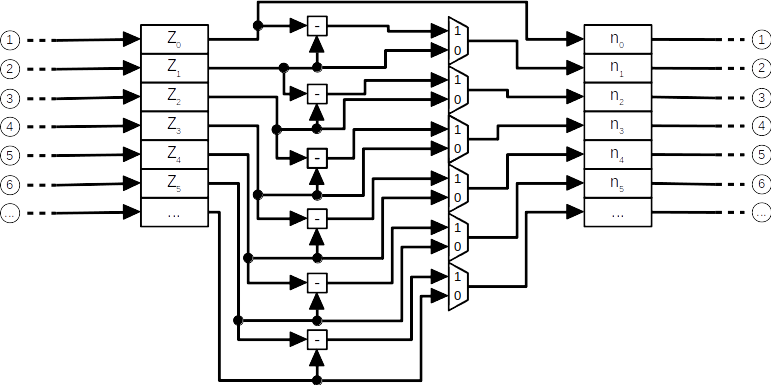
\includegraphics{pictures/title.png}}


%----------------  BFH tile page   -----------------------------------------
\maketitle
%------------ ABSTRACT        ----------------
\section*{ABSTRACT}

Interpolation is often key to perform analytical operations such as
\textit{Integration} and \textit{Derivation} which in turn are often key for
time critical applications or live analysis of data. One such interpolation
method is the Newton polynomial interpolation which uses the divided
difference in the Aitken-Neville recursion. This method consists of fairly
simple arithmetic operations and algorithms. Translating these algorithms into
hardware might prove to speedup the calculation of the Newton coefficients for
the interpolation polynomial.

\clearpage

%------------ TABLEOFCONTENTS ----------------
\tableofcontents

%------------ START MAIN PART ------------
\mainmatter

\section{Introduction}

Bringing a time discrete function, or rather measurements, into a time
continuous domain is often essential for analysis of time discrete data. To do
so, one can either approximate or interpolate. While approximation has
advantages such as being resistant to errors of random nature, interpolation
brings the advantage of being true to the original data. Unlike an
approximation, a interpolation can recall each data point with the
interpolating function.

Again one has a vast variety of interpolation methods at hand, each with their
pros and cons. One such method is the Newton interpolation, a high order
polynomial interpolation. These polynomials can be determined fairly
efficiently using the Aitken-Neville recursion with the divided difference.
This recursion yields the coefficients needed by a Newton polynomial for a
given dataset.

As analysis of measurement data is often performed while data is collected,
the speed of the interpolation algorithm is critical. One way of improving the
speed of algorithm is the implementation in hardware, as highly specific and
optimized hardware is usually faster than a generalized software implementation.

\textit{Outline:} Section 2 shows the mathematics behind the Newton
interplation, the Aitken-Neville recursion, and the divided difference.
Section 3 shows the chosen approach for the implementation in hardware based
on the previously discussed mathematics. Section 4 describes the resulting
hardware implementation while Section 5 discusses the limitations and further
aspects of the deduced hardware. Section 6 concludes the work.

\section{Methodology of Interpolation\footnote{This section is a summary of the
	Script \textit{Newton Polynomial Interpolation (Collocation)} of the
	Master lecture \textit{Numerical Analysis}}}

\subsection{The collocation problem}
There exists a vast variety of possible interpolation methods. One such method
is through collocation with a high-order polynomial, such as:

\begin{align}
	y(x) &= p(x) = c_0 + c_1 x^1 + c_2 x^2 + \dots
		+ c_{m-1} x^{m-1} + c_m x^m
			&(c_0, c_1, \dots c_m \in \mathbb{R}) \\
	\Rightarrow y(x_k) &= p(x_k) = y_k &(k = 0,1,2,3,\dots,n)
\end{align}

\textit{\textbf{Note:} The degree $m$ should be minimal, but the collocation
	conditions must be met.}

\begin{defn}
	Collocation: \textit{A single curve passing through all corresponding
		measurements.}
\end{defn}

A unique set of coefficients $c_0, c_1, c_2, \dots, c_m$ can be found using
elementary linear algebra if $m=n$. Though, this is proofs to be a very
inefficient method. Furthermore, this method is subject to significant numeric
instabilities.


\subsection{Aitken-Neville recursion}
An alternative method for finding the coefficients to the interpolating
polynomial is the Aitken-Neville recursion. Hereby the data is partitioned.
The \textit{global} polynomial terms are then determined using the relations
between different \textit{parial} polynomials.

\begin{defn}
	Aitken-Neville recursion: \textit{Finding the global polynomial through
		repetitive combination of ever smaller, partial polynomials.}
\end{defn}

This recursive algorithm can be represented in a tabular fashion.
\begin{table}[H]
	\centering
	\begin{tabular}{ r | l l l l l }
		$x_0$	& $y_0 = p_0$	&		&		&		& \\
		$x_1$	& $y_1 = p_1$	& $p_{01}$	&		&		& \\
		$x_2$	& $y_2 = p_2$	& $p_{12}$	& $p_{012}$	&		& \\
		$x_3$	& $y_3 = p_3$	& $p_{23}$	& $p_{123}$	& $p_{0123}$	& \\
		$x_4$	& $y_4 = p_4$	& $p_{34}$	& $p_{234}$	& $p_{1234}$	& $p_{01234} = p_4(x)$ \\
		$\vdots$ & $\vdots$	&		&		&		& \\
	\end{tabular}
	\caption{Visual representation of Aitken-Neville recursion: $p_{01}$ can
		be determined with $p_0$ and $p_1$, $p_{12}$ can be determined
		with $p_1$ and $p_2$. $p_{012}$ can then be determined with
		$p_{01}$ and $p_{12}$ and so forth.}
\end{table}


\subsection{Newton basis polynomials}
Using the Newton basis polynomials instead of the powers of $1, x^1, x^2, x^3,
\dots, x^m$ further increases the efficiency of the computational scheme for
resolving the collocation problem as it leads to a lower-triangular form of
the system of equations produced by polynomial interpolation.

The Newton basis polynomials are defined as such:
\begin{figure}[H]
	\centering
	\renewcommand{\figurename}{Equations}
	\begin{align*}
		\Pi_0(x) &= 1 \\
		\Pi_1(x) &= (x - x_0) \\
		\Pi_2(x) &= (x - x_0)(x - x_1) \\
		\Pi_3(x) &= (x - x_0)(x - x_1)(x - x_2) \\
		\Pi_4(x) &= (x - x_0)(x - x_1)(x - x_2)(x - x_3) \\
		\vdots \\
		\Pi_k &= (x - x_0)(x - x_1)(x - x_2)(x - x_3) \dots (x - x_{k-1}) \\
		\vdots \\
		\Pi_n &= (x - x_0)(x - x_1)(x - x_2)(x - x_3) \dots (x - x_{n-1})
	\end{align*}
	\caption{Newton basis polynomials for
		$\Pi_k(x) \quad (k = 0,1,2,\dots,n)$}
\end{figure}


Using the Newton basis polynomials for the collocation problem reduces the
system of equations to a single polynomial:
\begin{figure}[H]
	\centering
	\renewcommand{\figurename}{Equations}
	\begin{align}
		p(x) &= a_0 \Pi_0(x) + a_1 \Pi_1(x) + a_2 \Pi_2(x) + a_3 \Pi_3(x)
			+ \dots + a_m \Pi_m(x)
	\end{align}
	\caption{Resulting Newton polynomial to the degree $m$}
\end{figure}

Using more measurements for the collocation problem results in an increase of
the degree of the Newton polynomial:
\begin{figure}[H]
	\centering
	\renewcommand{\figurename}{Equations}
	\begin{align*}
		y_0 = p(x) &= a_0 \\
		y_1 = p(x) &= a_0 + a_1 \Pi_1(x) \\
		y_2 = p(x) &= a_0 + a_1 \Pi_1(x) + a_2 \Pi_2(x) \\
		\vdots \\
		y_k = p(x) &= a_0 + a_1 \Pi_1(x) + a_2 \Pi_2(x) + \dots + a_k \Pi_k(x) \\
		\vdots \\
		y_n = p(x) &= a_0 + a_1 \Pi_1(x) + a_2 \Pi_2(x) + \dots + a_n \Pi_n(x)
	\end{align*}
	\caption{Newton polynomials for $y_k(x) \quad (k = 0,1,2,\dots,n)$
		through application of Aitken-Neville recursion}
\end{figure}


\subsection{Bringing it all together}
Applying the Aitken-Neville recursion to the Newton polynomial leads to
following computational scheme. This is also known as the divided difference:
\begin{align}
	y(x_0, x_1, \dots, x_k) &= \frac{y(x_1, x_2, \dots, x_k) - y(x_0, x_1, \dots, x_{k-1})}
		{x_k - x_0} \quad (k = 0,1,2,\dots,n)
\end{align}

\begin{table}[H]
	\centering
	\begin{tabular}{ r | l }
	$k = 0$ & $y(x_0)$\\
	$k = 1$ & $\frac{y(x_1) - y(x_0)}{(x_1 - x_0)}$\\
	$k = 2$ & $\frac{y(x_1, x_2) - y(x_0, x_1)}{(x_2 - x_0)}$\\
	$k = 3$ & $\frac{y(x_1, x_2, x_3) - y(x_0, x_1, x_2)}{(x_3 - x_0)}$\\
	\end{tabular}
	\caption{Divided difference up to order 3}
\end{table}

\begin{defn}
	Divided Difference: \textit{Dividing the values of two points by the
		step size of said points. This is closely related to the
		derivative.}
\end{defn}

Following simple example demonstrates the computation of the divided
difference in tabular form:
\begin{table}[H]
	\centering
	\begin{tabular}{ l | l l l l }
	x	& y	& $\frac{\Delta y}{\Delta x}$	&		& \\ \hline
	$0$	& $1$	&			&			& \\
	$1$	& $1$	& $\frac{1-1}{1-0} = 0$	&			& \\
	$2$	& $2$	& $\frac{2-1}{2-1} = 1$	& $\frac{1-0}{2-0}$	& \\
	$4$	& $5$	& $\frac{3}{2}$		& $\frac{1}{6}$		& $\frac{-1}{12}$ \\
	\end{tabular}
	\caption{Example for determining the Newton coefficients through divided
		difference. The right-most value of each row is the Newton
		coefficient for given dataset: $a_0 = 1$, $a_1 = 0$, $a_2 =
		\frac{1}{2}$, $a_3 = \frac{-1}{12}$}
\end{table}

This example shows how the computation of the divided difference follows a
simple recursive algorithm. This is the algorithm, which was implemented in
hardware.


\subsection{Limitations}
The considerate algorithm is invariant to the order of the data and the time
deltas between each data point. Meaning the measurement intervals can vary and
the taken measurements can be fed in random order into the algorithm.

For this implementations these properties are limited: The measurements have
to be in a time-coherently order and must have a fixed measurement frequency.

\section{Implementation}

\subsection{Separation of the axis}

The first step to implement Aitken-Neville recursion for the Newton coefficients
in hardware is to separate the division in the divided difference into it's own
calculation. This has the advantage of separating the very costly operation of
the division from the recursive portion of the algorithm.

\subsection{Division}

It can then be proven that for equidistant measurements each column of the
table scheme of the divided difference shares the same denominator. This is
shown in following table:

\begin{table}[H]
	\centering
	\begin{tabular}{ l | l l l l l }
	\textbf{x}	& \textbf{y}	& $\frac{\Delta y}{\Delta x}$	&			&							& \\ \hline
	$1$	& $y_0$	&				&					&							& \\
	$2$	& $y_1$	& $\Delta_{01} \frac{1}{1}$	&					&							& \\
	$3$	& $y_2$	& $\Delta_{12} \frac{1}{1}$	& $\Delta_{012} \frac{\frac{1}{1}}{2}$	&							& \\
	$4$	& $y_3$	& $\Delta_{23} \frac{1}{1}$	& $\Delta_{123} \frac{\frac{1}{1}}{2}$	& $\Delta_{0123} \frac{\frac{\frac{1}{1}}{2}}{3}$	& \\
	$5$	& $y_4$	& $\Delta_{34} \frac{1}{1}$	& $\Delta_{234} \frac{\frac{1}{1}}{2}$	& $\Delta_{1234} \frac{\frac{\frac{1}{1}}{2}}{3}$	& $\Delta_{01234} \frac{\frac{\frac{\frac{1}{1}}{2}}{3}}{4}$ \\
	$\vdots$& $\vdots$	&			&					&							& \\
	\end{tabular}
	\caption{Divided difference with normed, equidistant measurements.}
\end{table}

This has several advantages:
\begin{itemize}
	\item The calculation of the denominator is reduced to a problem with
		linear proportion.
	\item These values can be predetermined an stored in a lookup-table.
\end{itemize}

Due to this property the denominator can be calculated iteratively with
following calculation scheme:

\begin{table}[H]
	\centering
	\begin{tabular}{ c c | c c | c c | c }
		$Z_1^{prev}$	& input	& $Z_1 - Z_2$	& $P_1^{\text{prev}}$	& $S_1 + S_2$		& $R^{\text{prev}}$	& $P_1 \cdot P_2$ \\
		$Z_2$		& $Z_1$	& $S_1$		& $S_2$			& $P_1$			& $P_2$			& $R$ \\ \hline
		1 & 2 & 1 & {\color{gray}0} & 1 & {\color{gray}1} & 1 \\
		2 & 3 & 1 & 1 & 2 & 1		& 2 \\
		3 & 4 & 1 & 2 & 3 & 2		& 6 \\
		4 & 5 & 1 & 3 & 4 & 6		& 24 \\
		5 & 6 & 1 & 4 & 5 & 24		& 120 \\
		6 & 7 & 1 & 5 & 6 & 120		& 720 \\
		7 & 8 & 1 & 6 & 7 & 720		& 5040 \\
		8 & 9 & 1 & 7 & 8 & 5040	& 40320 \\
	\end{tabular}
	\caption{Example of the algorithm with a normalized equidistant set of
		measurements. $S_2$ and $P_2$ need to be initialized with $0$
		and $1$ respectively.}
\end{table}

\lstinputlisting[language=python,caption=Python implementation of the calculation scheme]{implementation/x-demo.py}

\subsection{Difference}

The calculation of the nominator remains the same as divided difference with
the Aitken-Neville recursion though the division is no longer performed
reducing the calculation to a simple subtraction:

\begin{table}[H]
	\centering
	\begin{tabular}{ l | l l l l l }
	\textbf{x}	& \textbf{y}	& $\Delta y$		&			& \\ \hline
	$1$		& $y_0$		&			&			&			& \\
	$2$		& $y_1$		& $\Delta_{y_{01}}$	&			&			& \\
	$3$		& $y_2$		& $\Delta_{y_{12}}$	& $\Delta_{y_{012}}$	&			& \\
	$4$		& $y_3$		& $\Delta_{y_{23}}$	& $\Delta_{y_{123}}$	& $\Delta_{y_{0123}}$	& \\
	$5$		& $y_4$		& $\Delta_{y_{34}}$	& $\Delta_{y_{234}}$	& $\Delta_{y_{1234}}$	& $\Delta_{y_{01234}}$ \\
	$\vdots$	& $\vdots$	&			&			&			& \\
	\end{tabular}
	\caption{Reduction of the divided difference in the Aitken-Neville
		recursion to a difference for normed, equidistant data points.}
\end{table}

\lstinputlisting[language=python,caption=Python implementation of the calculation scheme]{implementation/y-demo.py}


\section{Results}

\subsection{Denominator}

\subsubsection{Lookup-table}
A big advantage of using a lookup-table is also the possibility make the data
point interval configurable. Figure \ref{fig:x-algo:non-norm} shows a
variation of implementation in figure \ref{fig:x-algo:lookup} with the
possibility of providing a custom interval.

\begin{figure}[H]
	\centering
	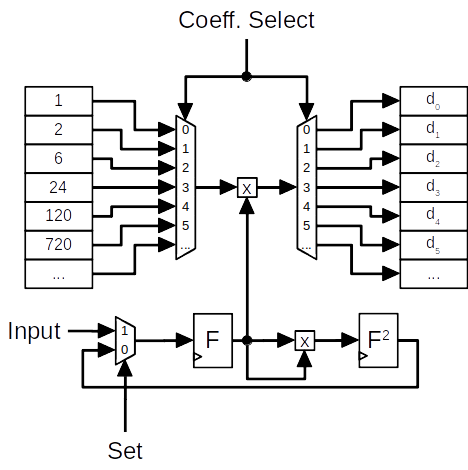
\includegraphics[width=.8\textwidth]{content/results/x-algo_lookup.png}
	\caption{Hardware algorithm to calculate the denominator with lookup-table for non-normalized intervals.}
	\label{fig:x-algo:lookup}
\end{figure}

The lookup table is a lot faster, but also uses the same amount of storage as
the dataset.

The lookup table for nine denominators is as follows:
\begin{table}[H]
	\centering
	\begin{tabular}{ c | c }
		\textbf{Index} & \textbf{Value} \\ \hline
		{\color{gray}0} & {\color{gray}1} \\
		1 & 1 \\
		2 & 2 \\
		4 & 6 \\
		5 & 24 \\
		5 & 120 \\
		6 & 720 \\
		7 & 5040 \\
		8 & 40320 \\
	\end{tabular}
	\caption{Denominator for up to column 8. Column \textit{0} contains the \textit{y} values.}
\end{table}


\subsubsection{On-the-fly generation}
As mentioned a lookup table requires a lot of storage. One way of mitigating
this problem is at the cost of speed and die space. Figure
\ref{fig:x-algo:on-the-fly} shows the hardware implementation for a on-the-fly
generation of the denominators.

\begin{figure}[H]
	\centering
	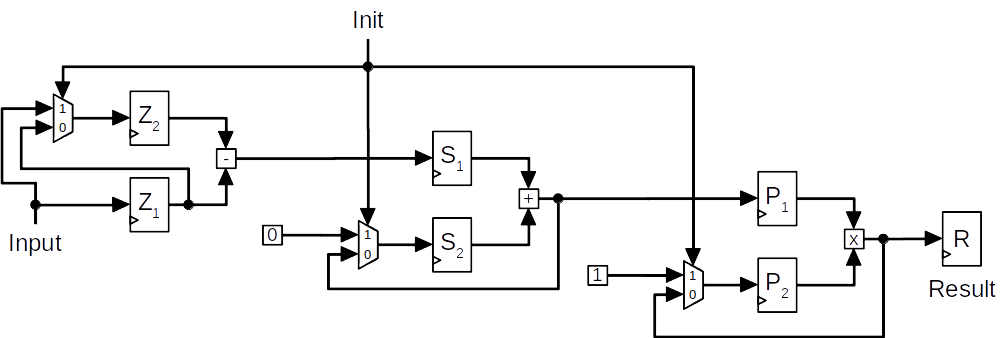
\includegraphics[width=.8\textwidth]{content/results/x-algo_on-the-fly.png}
	\caption{Hardware algorithm to calculate the denominator consecutively.}
	\label{fig:x-algo:on-the-fly}
\end{figure}

\subsection{Nominator}

\subsubsection{Iterative}
Figure \ref{fig:y-algo:iter} shows a iterative implementation for the
calculation of the nominator.

\begin{figure}[H]
	\centering
	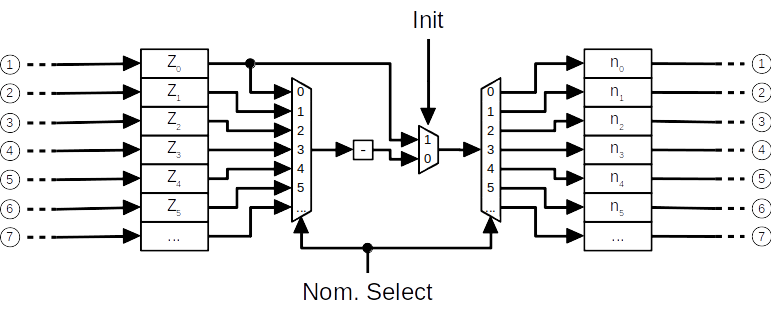
\includegraphics[width=.8\textwidth]{content/results/y-algo_iterative.png}
	\caption{Hardware algorithm to calculate the denominator consecutively.}
	\label{fig:y-algo:iter}
\end{figure}

Because of the triangular nature of the recursion, shown in table 6, the
register will hold the coefficients at the end of the computation reducing the
number of registers needed as the result does not have to be stored separately.

This implementation might prove to be to slow as the number of iterations is
proportional to $\frac{n^2}{2}$.



\subsubsection{Parallelization}
This implementation can easily parallelized to a certain extent to reduce the
quadratic nature to a linear nature. Figure \ref{fig:y-algo:parallel} shows a
parallelized version of the implementation.

\begin{figure}[H]
	\centering
	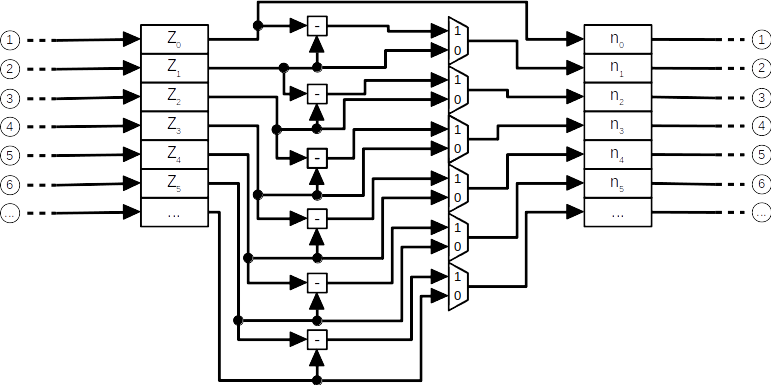
\includegraphics[width=.8\textwidth]{content/results/y-algo_parallel.png}
	\caption{Hardware algorithm to calculate the denominator with
		lookup-table for non-normed intervals.}
	\label{fig:y-algo:parallel}
\end{figure}



\section{Considerations}

\subsection{Limitation of dataset size}
The implemented solution is unable to handle new data points when the
registers are full. This is due to two reasons:

\begin{itemize}
	\item The hardware algorithm, especially the parallelized algorithm, is
		reliant on a given size of its registers, as this also
		determines the size of the multiplexers and the number of
		subtraction elements required. It must be noted that a more
		generalized and sophisticated implementation may be able to
		handle the arrival of new data points.

	\item Due to the quadratic nature of the underling mathematical problem,
		this solution will always exceed the available storage space.
		Depending on the situation, a segmentation of the data and
		therefore partial interpolation might mitigate this limitation.
\end{itemize}


\subsection{Hardware Improvements}

Following hardware optimizations can increase the speed of the implemented
algorithm:

\begin{itemize}
	\item \textbf{Signed Digits:} Using the signed digit notation can speed
		up the this implementation as it heavily relies on
		\textit{Addition/Subtraction.} The duration of these operations
		is then no longer proportional to the bus width.\footnote{Israel
		Koren, Computer Arithmetic Algorithms, 2.3 Signed-Digit Number
		Systems}

	\item \textbf{Booth's Algorithm:} The little amount of multiplication
		needed by the algorithm can be speed up using the Booth's
		algorithm to reduce the number of partial products. This
		algorithm itself heavily relies on
		\textit{Addition/Subtraction}. Again, the signed digit notation
		would be welcomed in this case. Though it must be mentioned that
		the compatibility of Booth's algorithm with the signed digit
		notation was not researched. It is unclear that the calculation
		scheme would still hold for the signed digit notation.
		\footnote{Israel Koren, Computer Arithmetic Algorithms,
		6.1 Reducing the Number of Partial Products}
\end{itemize}

\section{Conclusion}

Here presented are possible hardware implementation of the Aitken-Neville
recursion with the divided difference to calculate the coefficients of a
Newton interpolation polynomial. The proposed algorithm are designed with
speed and efficiency in mind, but are limited to the special case of
equidistant data points. The speed advantages of the hardware implementation
compared to a software implementation needs to be proven. It is noteworthy
that the Newton interpolation suffers from the Runge-Kutta phenomena which
makes this interpolation method inappropriate in many cases.


%------------ List of Figures ------------
\listoffigures

%------------ List of Tables -------------
\listoftables

%------------ List of Listings -----------
\lstlistoflistings

%------------ Index ----------------------
\clearpage
\printindex

\end{document}
